\documentclass[aspectratio=169]{beamer}
\usepackage[utf8]{inputenc}
\usepackage[english]{babel}
\usepackage{graphicx}
\usepackage{hyperref}
\hypersetup{
    colorlinks=true,
    linkcolor=blue,
    urlcolor=blue!70!black,
    citecolor=green!50!black
}
\usepackage{booktabs}
\usepackage{amsmath}
\usepackage{listings}
\usepackage{xcolor}

\usetheme{Madrid}
\usecolortheme{beaver}

\definecolor{codegreen}{rgb}{0,0.6,0}
\definecolor{codegray}{rgb}{0.5,0.5,0.5}
\definecolor{codepurple}{rgb}{0.58,0,0.82}
\definecolor{backcolour}{rgb}{0.95,0.95,0.92}

\lstdefinestyle{mystyle}{
    backgroundcolor=\color{backcolour},   
    commentstyle=\color{codegreen},
    keywordstyle=\color{magenta},
    numberstyle=\tiny\color{codegray},
    stringstyle=\color{codepurple},
    basicstyle=\ttfamily\footnotesize,
    breakatwhitespace=false,         
    breaklines=true,                 
    captionpos=b,                    
    keepspaces=true,                 
    numbers=left,                    
    numbersep=5pt,                  
    showspaces=false,                
    showstringspaces=false,
    showtabs=false,                  
    tabsize=2
}
\lstset{style=mystyle}

\title{Lab Quick Start: Introduction to AI and Python}
\subtitle{BMED365-2026: Computational Imaging, Modeling and AI in Biomedicine}
\author{BMED365}
\date{Spring 2026}

\begin{document}

\frame{\titlepage}

\begin{frame}{Overview}
    \tableofcontents
\end{frame}

\section{Introduction to the Course}
\begin{frame}{Welcome to BMED365}
    \begin{columns}
        \column{0.5\textwidth}
        \textbf{Course objectives:}
        \begin{itemize}
            \item Understand fundamental AI concepts.
            \item Apply machine learning to medical data.
            \item Get familiar with Python as a tool.
            \item Reflect on ethics and trustworthy AI.
        \end{itemize}
        
        \column{0.5\textwidth}
        \textbf{Structure:}
        \begin{itemize}
            \item \textbf{Lab 0:} ML with PyCaret (AutoML).
            \item \textbf{Lab 1:} Network analysis (PSN).
            \item \textbf{Lab 2:} Deep Learning (Images/ECG).
            \item \textbf{Lab 3:} Generative AI (LLM).
            \item \textbf{Lab 4:} Computational Imaging.
            \item \textbf{Lab 5:} Computational Modeling.
            \item \textbf{Projects:} Team + Individual.
        \end{itemize}
    \end{columns}
\end{frame}

\section{Python for Medical Professionals}
\begin{frame}{Why Python?}
    \begin{columns}
        \column{0.6\textwidth}
        Python has become the de-facto standard in AI and Data Science.
        \begin{itemize}
            \item \textbf{Readability:} Syntax resembles English pseudo-code.
            \item \textbf{Ecosystem:} Enormous libraries for everything from statistics to image analysis.
            \item \textbf{Community:} Great support and many examples online (Stack Overflow, ChatGPT).
        \end{itemize}
        \vspace{0.5cm}
        \textit{"Python is executable pseudocode."}
        
        \column{0.4\textwidth}
        \begin{block}{Prompt}
            \scriptsize\textit{"A friendly, stylized python snake coiling around a medical cross, 3d render, cute, clean background, high quality, medical blue and white color scheme."}
        \end{block}
        \centering
        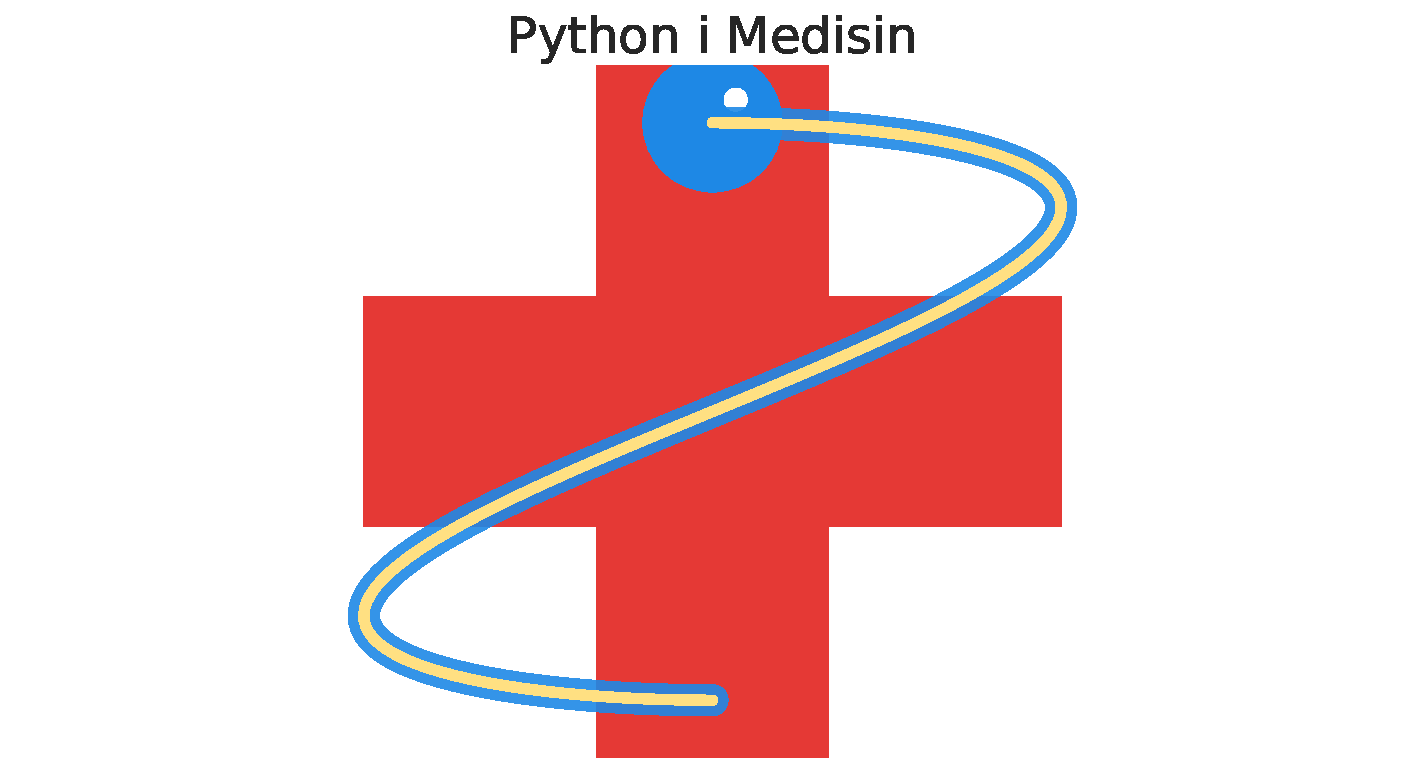
\includegraphics[width=0.6\textwidth]{images/python_medisin.pdf}
    \end{columns}
\end{frame}

\begin{frame}{Python vs. Other Languages}
    \begin{table}[]
        \centering
        \small
        \begin{tabular}{@{}lll@{}}
            \toprule
            \textbf{Language} & \textbf{Advantages} & \textbf{Disadvantages} \\ \midrule
            \textbf{Python} & Simple, AI standard, flexible & Slower than C++, GIL \\
            \textbf{R} & Excellent for statistics & Less support for Deep Learning \\
            \textbf{MATLAB} & Industry standard in engineering & Expensive, proprietary \\
            \textbf{C++} & Extremely fast & High learning curve, complex \\ \bottomrule
        \end{tabular}
    \end{table}
    \vspace{0.5cm}
    In BMED365, we use Python because the libraries (PyTorch, Scikit-learn) are best developed here.
\end{frame}

\section{Jupyter Notebooks}
\begin{frame}{The \href{https://jupyter.org/}{Jupyter Notebook} Environment}
    \begin{columns}
        \column{0.5\textwidth}
        A \textbf{Notebook} (.ipynb) combines:
        \begin{enumerate}
            \item \textbf{Executable code} (Python cells).
            \item \textbf{Rich text} (Markdown, LaTeX formulas).
            \item \textbf{Visualizations} (Plots directly in the document).
        \end{enumerate}
        This promotes \href{https://en.wikipedia.org/wiki/Reproducibility}{\textit{reproducible research}}.
        
        \column{0.5\textwidth}
        \begin{block}{Prompt}
            \scriptsize\textit{"Futuristic coding interface with visualization of medical data, holographic, blue and white theme, Python code snippets floating in the air, clean and modern."}
        \end{block}
        \centering
        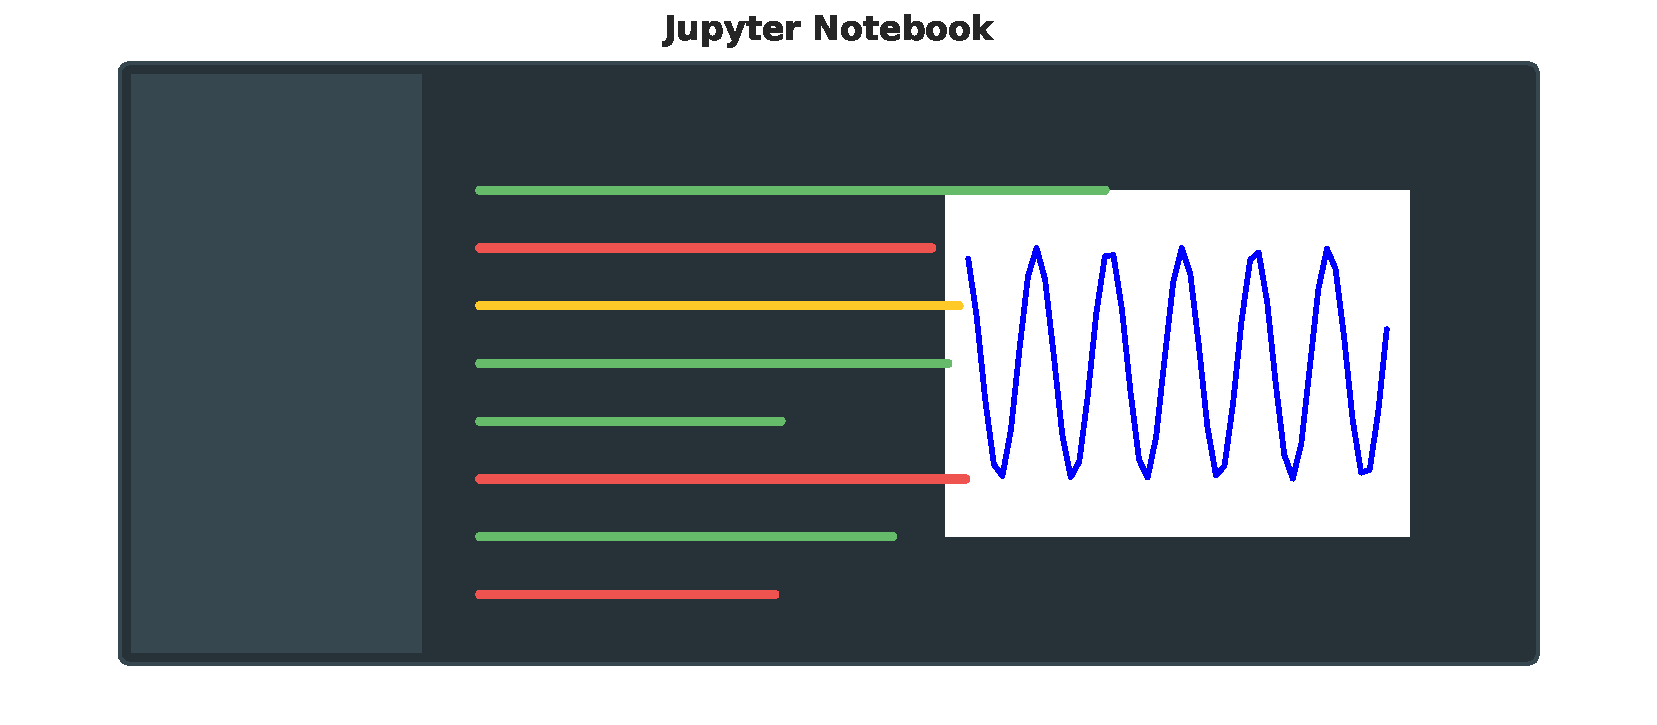
\includegraphics[width=0.6\textwidth]{images/coding_interface.pdf}
    \end{columns}
\end{frame}

\begin{frame}[fragile]{\href{https://www.markdownguide.org/}{Markdown} and \href{https://www.latex-project.org/}{LaTeX} in Jupyter}
    We can write formulas directly in text cells using \$:
    \vspace{0.5cm}
    
    \textbf{Example:}
    \begin{verbatim}
    The mean value is given by $\mu = \frac{1}{n} \sum x_i$
    \end{verbatim}
    
    \textbf{Result:}
    The mean value is given by $\mu = \frac{1}{n} \sum x_i$
    
    \vspace{0.5cm}
    This is useful for documenting mathematical methods in lab reports.
\end{frame}

\section{Important Libraries}
\begin{frame}{\href{https://numpy.org/}{NumPy}: Numerical Python}
    The foundation for all scientific computing in Python.
    \begin{itemize}
        \item Introduces \texttt{ndarray} (n-dimensional arrays).
        \item Much faster than regular Python lists due to C implementation and vectorization.
    \end{itemize}
    
    \vspace{0.5cm}
    \begin{block}{Mathematical operation}
        If $A$ and $B$ are matrices, \texttt{A * B} in NumPy is typically element-wise multiplication, while \texttt{A @ B} is matrix multiplication.
    \end{block}
\end{frame}

\begin{frame}[fragile]{\href{https://pandas.pydata.org/}{Pandas}: Data Processing}
    The main tool for tabular data (like Excel, but more powerful).
    
    \begin{columns}
        \column{0.5\textwidth}
        \begin{lstlisting}[language=Python]
import pandas as pd

# Read data
df = pd.read_csv('patient_data.csv')

# Inspect first rows
print(df.head())

# Statistics
print(df.describe())
        \end{lstlisting}
        
        \column{0.5\textwidth}
        \textbf{Important concepts:}
        \begin{itemize}
            \item \texttt{DataFrame}: The entire table.
            \item \texttt{Series}: A column.
            \item \texttt{.loc[]}: Get data by name.
            \item \texttt{.iloc[]}: Get data by index (position).
        \end{itemize}
    \end{columns}
\end{frame}

\begin{frame}{\href{https://matplotlib.org/}{Matplotlib} \& \href{https://seaborn.pydata.org/}{Seaborn}: Visualization}
    \begin{itemize}
        \item \textbf{Matplotlib:} The "grandfather" of plotting. Powerful, but can be verbose.
        \item \textbf{Seaborn:} Built on Matplotlib. More attractive default design, simpler for statistical plots.
    \end{itemize}
    
    \begin{center}
        \textit{A good visualization can replace a thousand numbers.}
    \end{center}
    We will use these to visualize confusion matrices, training curves, and feature importance.
\end{frame}

\section{Notebook Walkthrough}
\begin{frame}{Overview of `quickstart-ai-python.ipynb`}
    The notebook is divided into the following sections:
    \begin{enumerate}
        \item \textbf{Python Basics:} Variables, lists, loops, functions.
        \item \textbf{NumPy:} Vectors and matrices.
        \item \textbf{Pandas:} Load and explore a "Heart Disease" dataset.
        \item \textbf{Visualization:} Plotting histograms and correlations.
        \item \textbf{Scikit-learn intro:} A simple linear regression model.
    \end{enumerate}
\end{frame}

\begin{frame}[fragile]{Tips for Lab Work}
    \begin{itemize}
        \item \textbf{Run cells in order!} Variables must be defined before they are used.
        \item \textbf{Tab completion:} Press \texttt{Tab} to see available functions.
        \item \textbf{Help:} Use \texttt{?} after a function for documentation.
        \begin{lstlisting}[language=Python]
pd.read_csv?
        \end{lstlisting}
        \item \textbf{Restart Kernel:} If things get stuck, restart the kernel (Kernel $\rightarrow$ Restart).
    \end{itemize}
\end{frame}

\begin{frame}{The Road Ahead}
    When you are finished with the quick start, you are ready for \textbf{Lab 0}, where we will begin with real machine learning using \href{https://pycaret.org/}{PyCaret}.
    
    \vspace{1cm}
    \centering
    \textbf{Good luck with coding!}
\end{frame}

\end{document}
